%%% Работа с русским языком
\usepackage{cmap}					% поиск в PDF
\usepackage{mathtext} 				% русские буквы в формулах
\usepackage[T2A]{fontenc}			% кодировка
\usepackage[utf8]{inputenc}			% кодировка исходного текста
\usepackage[russian]{babel}	% локализация и переносы

%%% Дополнительная работа с математикой
\usepackage{amsmath,amsfonts,amssymb,amsthm,mathtools} % AMS
\usepackage{icomma} % "Умная" запятая: $0,2$ --- число, $0, 2$ --- перечисление

%% Номера формул
%\mathtoolsset{showonlyrefs=true} % Показывать номера только у тех формул, на которые есть \eqref{} в тексте.
%\usepackage{leqno} % Немуреация формул слева

%% Шрифты
\usepackage{euscript}	 % Шрифт Евклид
\usepackage{mathrsfs} % Красивый матшрифт

%%% Свои команды
\DeclareMathOperator{\sgn}{\mathop{sgn}}

%% Поля
\usepackage[left=2cm,right=2cm,top=2cm,bottom=2cm,bindingoffset=0cm]{geometry}

%% Русские списки
\usepackage{enumitem}
\makeatletter
\AddEnumerateCounter{\asbuk}{\russian@alph}{щ}
\makeatother

%%% Работа с картинками
\usepackage{graphicx}  % Для вставки рисунков
\graphicspath{{images/}{images2/}}  % папки с картинками
\setlength\fboxsep{3pt} % Отступ рамки \fbox{} от рисунка
\setlength\fboxrule{1pt} % Толщина линий рамки \fbox{}
\usepackage{wrapfig} % Обтекание рисунков и таблиц текстом

%%% Работа с таблицами
\usepackage{array,tabularx,tabulary,booktabs} % Дополнительная работа с таблицами
\usepackage{longtable}  % Длинные таблицы
\usepackage{multirow} % Слияние строк в таблице

%% Красная строка
\setlength{\parindent}{2em}

%% Интервалы
\linespread{1}
\usepackage{multirow}

%% TikZ
\usepackage{tikz}
\usetikzlibrary{graphs,graphs.standard}

%% Верхний колонтитул
% \usepackage{fancyhdr}
% \pagestyle{fancy}

%% Перенос знаков в формулах (по Львовскому)
\newcommand*{\hm}[1]{#1\nobreak\discretionary{}
	{\hbox{$\mathsurround=0pt #1$}}{}}

%% дополнения
\usepackage{float} %Добавляет возможность работы с командой [H] которая улучшает расположение на странице
\usepackage{gensymb} %Красивые градусы
\usepackage{caption} % Пакет для подписей к рисункам, в частности, для работы caption*

% подключаем hyperref (для ссылок внутри  pdf)
\usepackage[unicode, pdftex]{hyperref}

%%% Теоремы
\theoremstyle{plain}                    % Это стиль по умолчанию, его можно не переопределять.
\renewcommand\qedsymbol{$\blacksquare$} % переопределение символа завершения доказательства

\newtheorem{theorem}{Теорема}[section] % Теорема (счетчик по секиям)
\newtheorem{proposition}{Утверждение}[section] % Утверждение (счетчик по секиям)
\newtheorem{definition}{Определение}[section] % Определение (счетчик по секиям)
\newtheorem{corollary}{Следствие}[theorem] % Следстиве (счетчик по теоремам)
\newtheorem{problem}{Задача}[section] % Задача (счетчик по секиям)
\newtheorem*{remark}{Примечание} % Примечание (можно переопределить, как Замечание)
\newtheorem{lemma}{Лемма}[section] % Лемма (счетчик по секиям)

\newtheorem{example}{Пример}[section] % Пример
\newtheorem{counterexample}{Контрпример}[section] % Контрпример
\newcommand{\defeq}{\stackrel{def}{=}} % по определению
\newcommand{\defarr}{\stackrel{def}{\Rightarrow}} % следует из определения
\DeclareMathOperator{\Tr}{trace}

\begin{document}

\section*{Билет 1}
\subsection*{Уравнение Бернулли}

\begin{definition}
	Д.у. вида $ \boxed{y' + a(x)\cdot y = y^r \cdot f(x)}^{\eqnum\label{eq:Ber}} $, где $ a(x), f(x) \in C^1, r \in \mathbb{ R }, r \neq 1$ называется уравнением Бернулли. \\
\end{definition}

\begin{proposition} %% тут бы добавить расширение для переноса символов на новую строку, чтобы не приходилось дублировать стрелку 
	Если $ r > 0 $, то $ y \equiv 0 $ - тривиальное решение. Пусть $ y \neq 0$, разделим ДУ на $ y^r \Rightarrow \frac{ y' }{ y^r } + a(x) \cdot y^{ 1-r } = f(x).$ Замена: $ u(x) = y^{ 1-r } \Rightarrow u' = ( 1-r ) \cdot y^{ -r } \cdot y' \Rightarrow$ \\ $\Rightarrow \underbracket{ \frac{ 1 }{ 1-r } \cdot u' + a(x)\cdot u = f(x) }$ - свелось к линейному уравнению. 
\end{proposition}

\subsection*{Уравнение Риккати}

\begin{definition}
	Д.у. вида $ \boxed{y' + a(x) \cdot y^2 + b(x) \cdot y + c(x)}^{\eqnum\label{eq:Ric}} $, где $a(x),  b(x) \in C^1_{I(x)},  \\ c(x) \in C_{I(x)}$ называется уравнением Риккати. 
\end{definition}

\begin{proposition}	
	В общем случае уравнение Риккати не допускает решений в квадратурах, однако, если известно некоторое решение $ y = \varphi (x) $, то сделав замену $ y = u + \varphi $, получаем: $ \varphi' = u \varphi^2 + b\varphi + c $ \\ $ \varphi' + u' = u\varphi^2 + 2a\varphi u + au^2 + b\varphi + bu + c \Rightarrow u' = au^2 + (2a\varphi + b)u $ - свелось к уравнению Бернулли.
\end{proposition}

\subsection*{Методы понижения порядка дифференциальных уравнений}
\begin{proposition}

	Рассмотрим множество преобразований плоскости \\ $ \boxed{\bar{x} = \varphi(x,y,\lambda), \bar{y} = \psi (x,y,\lambda)}^{\eqnum\label{eq:trans}} $. В \eqref{eq:trans} каждому $ \lambda \in \mathcal{ D }  \subset \mathbb{ R } $ соответствует некоторое преобразование, например, $ \bar{x} = \lambda x, \bar{y} = \lambda y, \lambda > 0 $ - гомотетия. Множество преобразований \eqref{eq:trans}  является группой преобразований, если оно содержит любую композицию \eqref{eq:trans} , т.е. 
	$ \exists \lambda_0 : \varphi(\varphi(x,y,\lambda_1), \psi(x,y,\lambda_2)) = \varphi(x,y,\lambda_0) $, содержит тожедественное преобразование, т.е. $ \exists \lambda_0: \varphi(x,y,\lambda_0) = x; \ \psi(x,y,\lambda_0) = y $, и вместе с любым преобразованием содержит и обратное: $ \forall \lambda \in \mathcal{D} \colon  \exists \ \lambda_0 \colon x = \bar{ \varphi } (\bar{x}, \bar{y}, \lambda_0); \ y = \bar{ \psi } (\bar{x}, \bar{y}, \lambda_0) $ \\
	Т.о. если \eqref{eq:trans} - группа, то $ x = \bar{ \varphi } (\bar{x}, \bar{y}, \lambda), \ y = \bar{ \psi } (\bar{x}, \bar{y}, \lambda);$ если в ДУ $ y' = f(x,y)$ осуществить переход к новым координатам, то \\
	$$
	\frac{dy}{dx} = \frac{ \psi'_{ \bar{x} } d\bar{x} +  \psi'_{ \bar{y} } d\bar{y} }{ \varphi'_{\bar{x}} d\bar{x} +  \varphi'_{\bar{y}} d\bar{y}} = f(\bar{ \varphi }(\bar{x}, \bar{y}, \lambda), \bar{ \psi }(\bar{x}, \bar{y}, \lambda)) = \tilde{f}(\bar{x}, \bar{y}, \lambda) \Rightarrow
	$$	
	\begin{equation} \label{eq:def}
	\Rightarrow \frac{ \psi'_{ \bar{x} } + \psi'_{ \bar{y} } \cdot \frac{d\bar{y}}{d\bar{x}} }{ \varphi'_{\bar{x}} +  \varphi'_{\bar{y}} \cdot \frac{d\bar{y}}{d\bar{x}} } = \tilde{f}(\bar{x}, \bar{y}, \lambda) \Rightarrow \frac{d\bar{y}}{d\bar{x}} = \frac{\tilde{f} \cdot \varphi'_{\bar{x}} - \psi'_{\bar{x} }}{\psi'_{\bar{y}} - \tilde{f} \cdot \varphi'_{\bar{y}}}
	\end{equation}  
	
	\noindent\eqref{eq:def} является записью $ y' = f(x,y) $ в новых координатах. Говорят, что $ y' = f(x,y) $ допускает группу $ x =\bar{ \varphi }(\bar{x}, \bar{y}, \lambda), \ y = \bar{ \psi } (\bar{x}, \bar{y}, \lambda)$, если оно не изменяется при переходе к новым переменным, т.е. $ \frac{d\bar{y}}{d\bar{x}} = f(\bar{x}, \bar{y}) $
\end{proposition}

\begin{corollary}
	Рассматриваем уравнения вида $ \boxed{F(x, y, y', y'') = 0}^{\eqnum\label{eq:F0}} $ \\
	\begin{enumerate}
		\item $\boxed{F(x,y'',y') = 0}^{\eqnum\label{eq:F1}}$ Замена $y'(x) = v(x) \Rightarrow y''(x) = v'(x) \ \text{и }   \eqref{eq:F1}$ в этом случае имеет вид $ F(x, v(x), v'(x)) = 0 \xrightarrow[\text{решаем}]{} V(x) = y(x,c_1)$. Тогда решение $\eqref{eq:F1}$ запишется в виде $ \frac{dy}{dx} = g(x, c_1) \Rightarrow y(x) = c_2 + \int g(x,c_1)dx$. Заметим, что $ \eqref{eq:F1} $ допускает группу сдвига $ x = \bar{x}, \  y = \bar{y} + y_0 $
		\item $\boxed{F(y,y',y'') = 0}^{\eqnum\label{eq:F2}} \ (\text{не содержит явно x}) $.  Замена: $ y' = V(y),$ тогда \\
		 $y'' = \frac{dV}{dx} = \frac{dV}{dy}\frac{dy}{dx} = V\frac{dV}{dy} \Rightarrow F(y, V, y\frac{dV}{dy}) = 0$ - ДУ первого порядка. \\
		 Решение $ V(y) = g(y,c_1) \Rightarrow  \frac{dy}{dx} = g(y,c_1) \Rightarrow $ Решение $\eqref{eq:F2}$: $ \int \frac{dy}{g(y,c_1)} = x + c_2. $ \\
		 Заметим, что $ \eqref{eq:F2} $ допускает группу сдвигов $ x = \bar{x} + x_0 $, $ y = \bar{y} $
		 \item $ \boxed{F(x, y'',y',y) = 0 \  \text{и} \ F - \text{однородная степени m по y'', y', y} }$, т.е. $ \forall \lambda > 0 \rightarrow$ \\
		  $F(x, \lambda y'', \lambda y', \lambda y) = \lambda^m \cdot F(x, y'', y', y) $. В таком случае ДУ допускает группу \\ 
		  $ x = \bar{x}, y = \lambda \bar{y}$. Замена: $z(x) = \frac{y'}{y} \Rightarrow y' = z(x)y$ \\ 
		  $ \Rightarrow y'' = z'  y + zy' = z'y + z^{2}y = y \cdot (z' + z^2) \Rightarrow F(x, y, zy, y(z' + z^2)) = 0$ \\
		  $ \Rightarrow y^m \cdot F(x, 1, z, z' + z^2) = 0
		  $ - относительно z имеем ур-ние первого порядка. \\
		  Если его решение $z(x) = g(x, c_1),$ то $\frac{y'}{y} = g(x, c_1) \Rightarrow \frac{dy}{y} = g(x, c_1)dx \Rightarrow$ \\ 
		  $ \ln|y| = \int g(x, c_1)dx + c_2 $
		  \item[4*.] Будем говорить, что функция $ F(x, y, y'', ..., y^{(n)})$ является квазиоднородной функцией степени $ r $, если $ \exists \alpha \in \mathbb{ R }: \forall \lambda > 0: F(\lambda x, \lambda^{\alpha}y, \lambda^{\alpha - 1}y', ..., \lambda^{\alpha - n}y^{(n)} ) =$ \\ $ = \lambda^r \cdot F(x, y, ..., y^{(n)}). $ \\
		  Рассмотрим множество преобразований:
		  \begin{equation} \label{eq:conv}
		  \left\{
		  \begin{aligned} 
		  	x &= \lambda \bar{x}  \\
		  	y &= \lambda^{\alpha} \bar{y}\\   
		  \end{aligned}
		  \right.\text{,}  \quad  \text{где } \lambda > 0                                            
		  \end{equation}

		  Такое множество преобразований перепишем в виде: 
		 \[
			\left\{
			\begin{aligned}
				x &= e^{\beta} \cdot \bar{x}  \\
				y &= e^{\alpha \beta} \bar{y} \\   
			\end{aligned}
			\right.                                                          
		\]
		Если F в $\eqref{eq:F2}$ является квазиоднородной, то $\eqref{eq:F2}$ допускает группу растяжений $\eqref{eq:conv}$: \\
		\[
			\boxed{F(x, y'', y', y) = 0} \xrightarrow[\text{преобр.}]{} F(\lambda \bar{x}, \lambda^{\alpha} \bar{y}, \lambda^{\alpha - 1} \bar{y'}, \lambda^{\alpha - 2} \bar{y''}) = \lambda^{r} \cdot F(\bar{x}, \bar{y}, \bar{y'}, \bar{y''}) = 0
		\]
		\[
			\Downarrow
		\]
		\[
		 	F(\bar{x}, \bar{y}, \bar{y'}, \bar{y''}) = 0
		\]
		\ \\
	    \[
		\text{Замена: }\left\{
		\begin{aligned}
			x &= e^{t}  \\
			y &= z(t) \cdot e^{2t}\\   
		\end{aligned}
		\right. \quad
		\Rightarrow  \quad y'_x = \frac{y'_t}{x'_t} = \frac{z'_t \cdot e^{\alpha t} +  z \cdot \alpha \cdot e^{\alpha t}}{e^t} =  e^{(\alpha  -  1)t} \cdot (z'_t  + \alpha z)                                              
		\]
		\[
		  \Downarrow
		\]
		\[
			y''_{xx} = \frac{(y'_x)'_t}{x'_t} = \frac{(\alpha - 1) \cdot e^{(\alpha - 1)t} \cdot (z'_t + \alpha z) + e^{(\alpha - 1)t} \cdot (z''_{tt} + \alpha z'_t)}{e^t} = 
		\]	
		\[	
			= e^{(\alpha - 2)t} \cdot (z''_{tt} + (2\alpha - 1)\cdot z'_t + \alpha \cdot (\alpha - 1)z)
		\]
		\[
		  \Downarrow
		\]
		\[
			F(e^t; z \cdot e^{\alpha t}; e^{(\alpha - 1)t} \cdot (z'_t + \alpha z); e^{(\alpha - 2)t}(z''_{tt} + (2\alpha - 1)z'_t + \alpha \cdot (\alpha - 1)z) ) =
		\]
		\[
			= e^{rt} \cdot F(1; z; z'_t + \alpha z; z''_{tt} + (2\alpha - 1)z'_t + \alpha \cdot (\alpha - 1)z) = 0 \text{ -  не содерж. x, т.е. свелось к случаю 2}
		\]
	\end{enumerate}
\end{corollary}
\newpage
\subsection*{Метод введения параметра для уравнения первого порядка, не разрешенного относительно производной.}
\begin{proposition}
	Рассмотрим $ \boxed{F(x,  y, y') = 0}^{\eqnum\label{eq:F4}} \ $, где $ F(x, y, y') $ как функция трёх переменных является непрерывно дифференцируемой в области $ G \subset \mathbb{ R }^3 $ \\
	Решение уравнения $F(x, y, y') = 0 $ будем представлять как кривую в параметрическом виде: \\
	\begin{equation} \label{eq:int}
	\gamma: \	\left\{
	\begin{aligned}
		x &= \varphi(t)  \\
		y &= \psi(t) \\   
	\end{aligned}
	\right. \ t \in [t_1, t_2], \ \varphi(t), \psi(t) \in C^1_{[t_1, t_2]}                                             
	\end{equation}
	Кривая \eqref{eq:int}, является интегральной кривой \eqref{eq:F4} $ \Rightarrow $ \\
	\begin{equation} \label{eq:F5}
	 \Rightarrow F\left(\varphi(t), \psi(t), \frac{\psi'_t}{\varphi'_t}\right) = 0 \ \ \forall t \in [t_1, t_2] 
	\end{equation}
	Будем решать эквивалентную систему положив $ p = \frac{dy}{dt} $: 
	\begin{equation} \label{eq:Fs}
		\left\{
		\begin{aligned}
			&F(x, y, p) = 0  \\
			&dy = pdx \\   
		\end{aligned}
		\right.                                                          
	\end{equation}
\end{proposition}

\begin{proposition}
	Уравнение \eqref{eq:F4} эквивалентно системе \eqref{eq:Fs}.
\end{proposition}

\begin{proof}
	Пусть $ \gamma $ - интегр. кривая \eqref{eq:F4}. Положим $ p = \frac{\psi'}{\varphi'} = \frac{dy}{dx} $ - второе уравнение в системе \eqref{eq:Fs} выполнено, а первое выполнено в силу подстановки в \eqref{eq:F5}. Обратно, пусть $x(t) = \varphi(t), \ y(t) = \psi(t), p$ - решение \eqref{eq:F5}. $ \Rightarrow$ Из второго уравнения системы:\\ 
	$ p = \frac{\psi'_t}{\varphi'_t} \rightarrow $ Подставляем в первое уравнение системы и получаем само уравнение \eqref{eq:F5}\\
\end{proof}

\begin{proposition}
	Рассмотрим метод решения \eqref{eq:F4}, который называется методом введения параметра. \\
	Первое ур-ние в системе \eqref{eq:Fs} рассмотрим как задающее в $\mathbb{ R }^3_{(x, y, p)} $ гладкую поверхность S, для которой параметрическое представление имеет вид:
	\begin{figure}[!h]
		\centering
		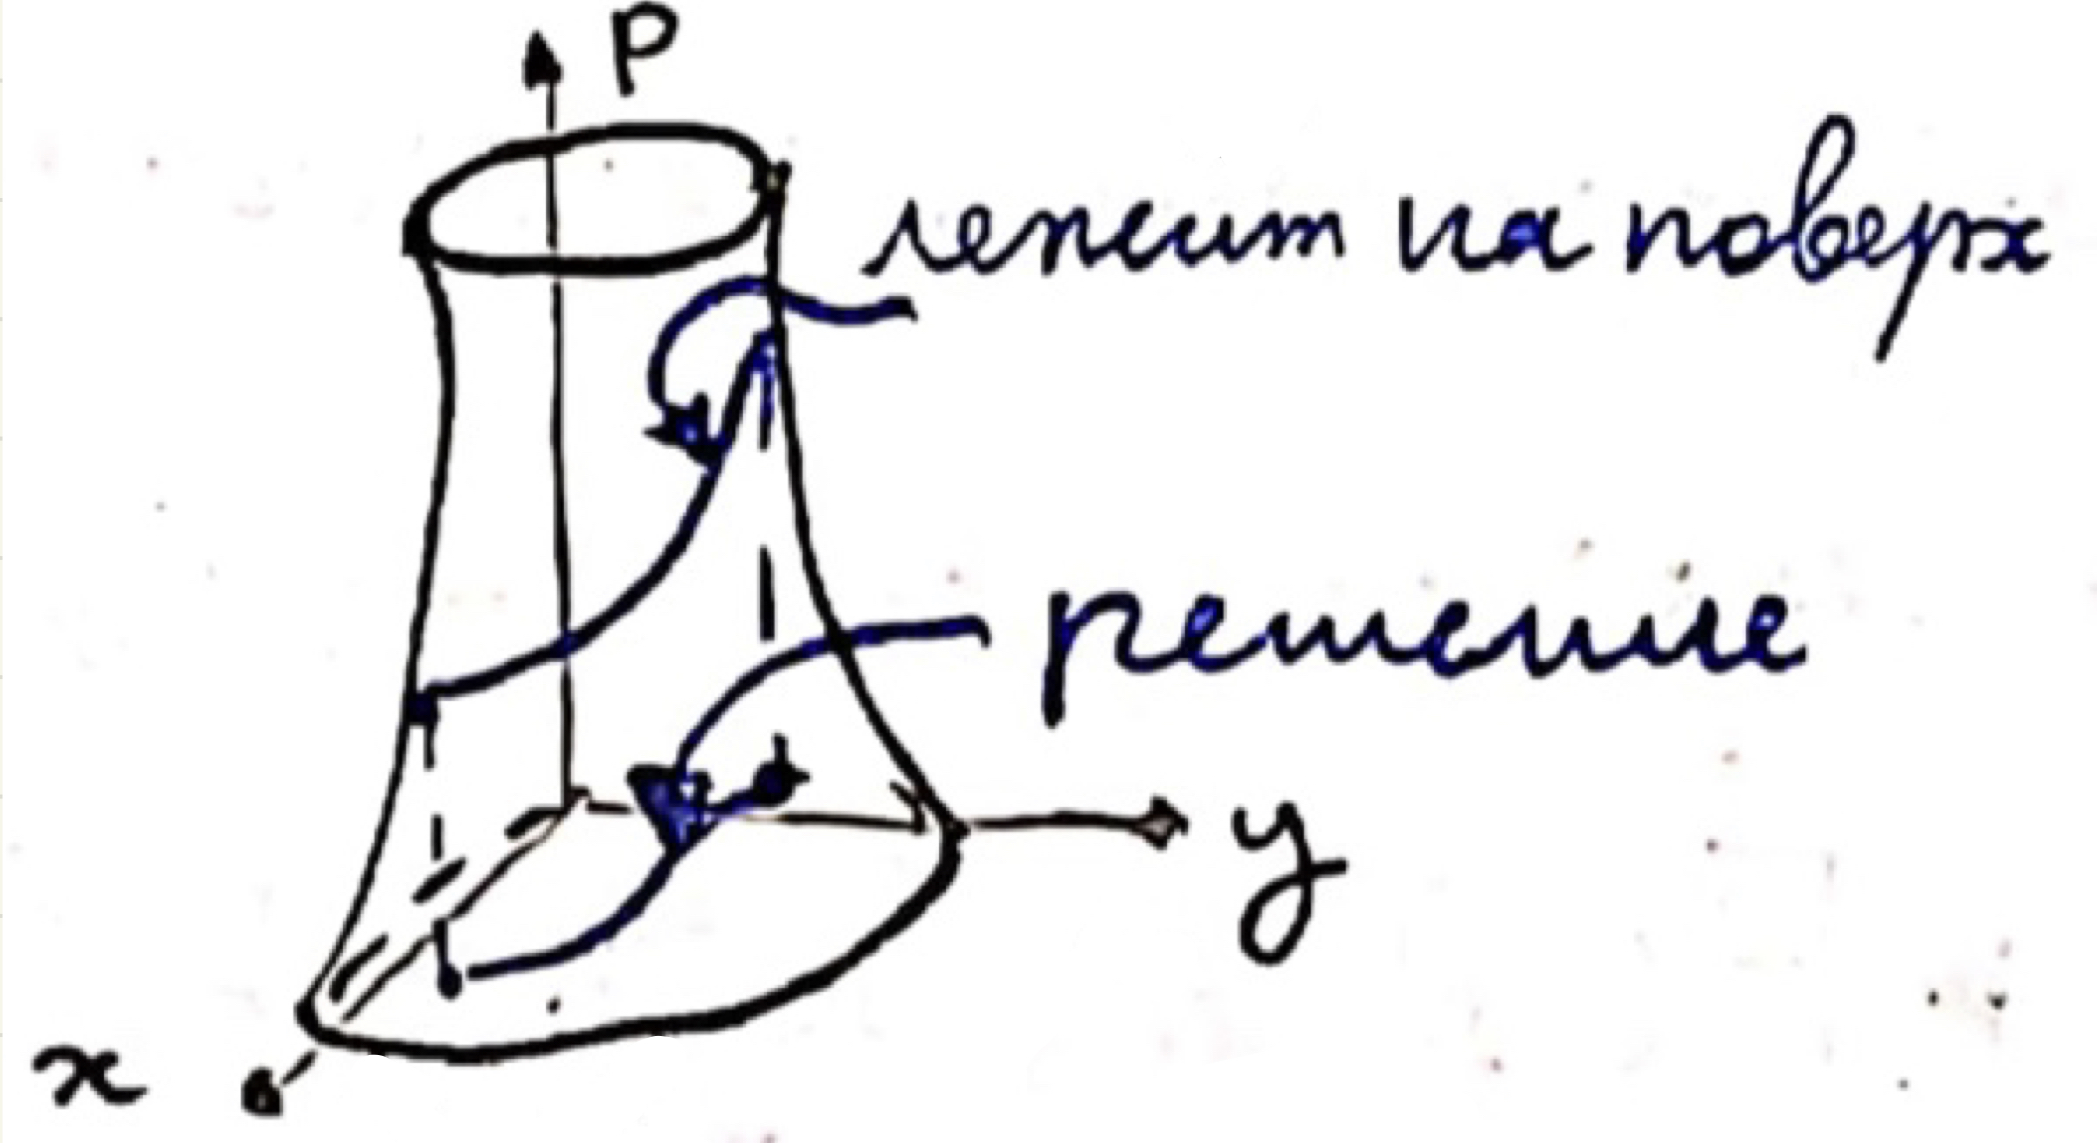
\includegraphics[width = 0.25\textwidth]{image_1.jpeg}
	\end{figure}	
	\[
	\left\{
	\begin{aligned}
		x &= \varphi(u, v)  \\
		y &= \psi(u, v) \\   
		p &= \chi(u, v) \\
	\end{aligned}
	\right.   
	\Rightarrow  F(\varphi(u, v); \psi(u, v); \chi(u, v)) \equiv 0                                                   
	\]
	\[
		\text{Потребуем, чтобы rank}
		\begin{pmatrix}                               
			\dfrac{\delta\varphi}{\delta u} & \dfrac{\delta \psi}{\delta u} & \dfrac{\delta \chi}{\delta u} \\
			\\
			\dfrac{\delta\varphi}{\delta v} & \dfrac{\delta \psi}{\delta v} & \dfrac{\delta \chi}{\delta v}
		\end{pmatrix} = 2, \ \forall u, v \in G \text{ т.е. S была простой гладкой пов.}
	\]
	Тогда остаётся удовлетворить второму уравнению системы \eqref{eq:Fs}: \\
	\begin{equation} \label{eq:F6}
		\frac{\delta \psi}{\delta u} du + \frac{\delta \psi}{\delta v} dv = \chi \cdot \left(\frac{\delta \varphi}{\delta u}du + \frac{\delta \varphi}{\delta v}dv\right) \Rightarrow \left( \frac{\delta \psi}{\delta u} - \chi \frac{\delta \varphi}{\delta v} \right) du = \left(\chi \frac{\delta \varphi}{\delta v} - \frac{\delta \psi}{\delta v} \right) dv
	\end{equation}
	Если $ P(u, v) \neq 0 \ \forall (u,v) \in G$, то из \eqref{eq:F6} получаем Д.У.: $ \dfrac{du}{dv} = \dfrac{Q(u, v)}{P(u, v)} $
	\[
		\text{Его решение} \  u = u(v, c),  \text{тогда } \left\{
		\begin{aligned}
			x &= \varphi(u(v, c), v) = x(v, c)  \ \text{ - является параметрическим}\\
			y &= \psi(u(v, c), v) = y(v, c) \ \ \text{ представлением  решения \eqref{eq:F4}}\\   
		\end{aligned}
		\right.   
	\]
	\\ 
	Если же существует связь между $u$ и $v$: $ u = f(v), P(f(v), v) = Q(f(v), v) = 0 \ \forall v \in G$, то $ u = f(v) $ явл. решением $ \left(\chi \frac{\delta \varphi}{\delta v} - \frac{\delta \psi}{\delta v} \right) dv $, а 
	\[
	\left\{
	\begin{aligned}
		x &= x(v)\\
		y &= y(v)\\   
	\end{aligned}
	\right.   \
	\text{ - явл. решением } \eqref{eq:F6}
	\]
\end{proposition}
	
\end{document}